\documentclass[xcolor=dvipsnames]{beamer}
\usetheme{Madrid}
\useoutertheme{miniframes} % Alternatively: miniframes, infolines, split
\useinnertheme{circles}

\definecolor{UBCblue}{rgb}{0.31, 0.055, 0.318} % UBC Blue (primary)
\definecolor{UBCgrey}{rgb}{0.9176, 0.6745, 0.2471} % UBC Grey (secondary)

\setbeamercolor{palette primary}{bg=UBCblue,fg=white}
\setbeamercolor{palette secondary}{bg=UBCblue,fg=white}
\setbeamercolor{palette tertiary}{bg=UBCblue,fg=white}
\setbeamercolor{palette quaternary}{bg=UBCblue,fg=white}
\setbeamercolor{structure}{fg=UBCblue} % itemize, enumerate, etc
\setbeamercolor{section in toc}{fg=UBCblue} % TOC sections

% Override palette coloring with secondary
\setbeamercolor{subsection in head/foot}{bg=UBCgrey,fg=white}
\usepackage{parskip}
\usepackage{caption}
\usepackage{url}
\usepackage{multicol}
\usepackage{amsmath}
\usepackage{esint}
\usepackage{amsfonts}
\usepackage{tikz}
\usetikzlibrary{decorations.pathmorphing}
\usepackage{amsmath,amssymb}
\usepackage{geometry}
\usepackage{colortbl}
\usepackage{xcolor}
\usepackage{mathtools}
\usepackage{amsmath,amssymb}
\usepackage[english]{babel}
\usepackage[utf8]{inputenc}
\usepackage{tabularx}
\usepackage{hyperref}
\usepackage{csquotes}
\usetheme{Madrid}
\newcommand{\source}[1]{\caption*{Source: {#1}} }
\title{Pour une science de la recherche - Séance 1}
\subtitle{Introduction à la structure et au rôle de la recherche}
\author{Valentin Auplat}
\date{}
\usepackage{tikz}
\usepackage{graphicx}
\logo{
	\vspace{5.2cm} % Ajustement vertical
	\hspace{6cm}    % Ajustement horizontal
	\raisebox{1cm}{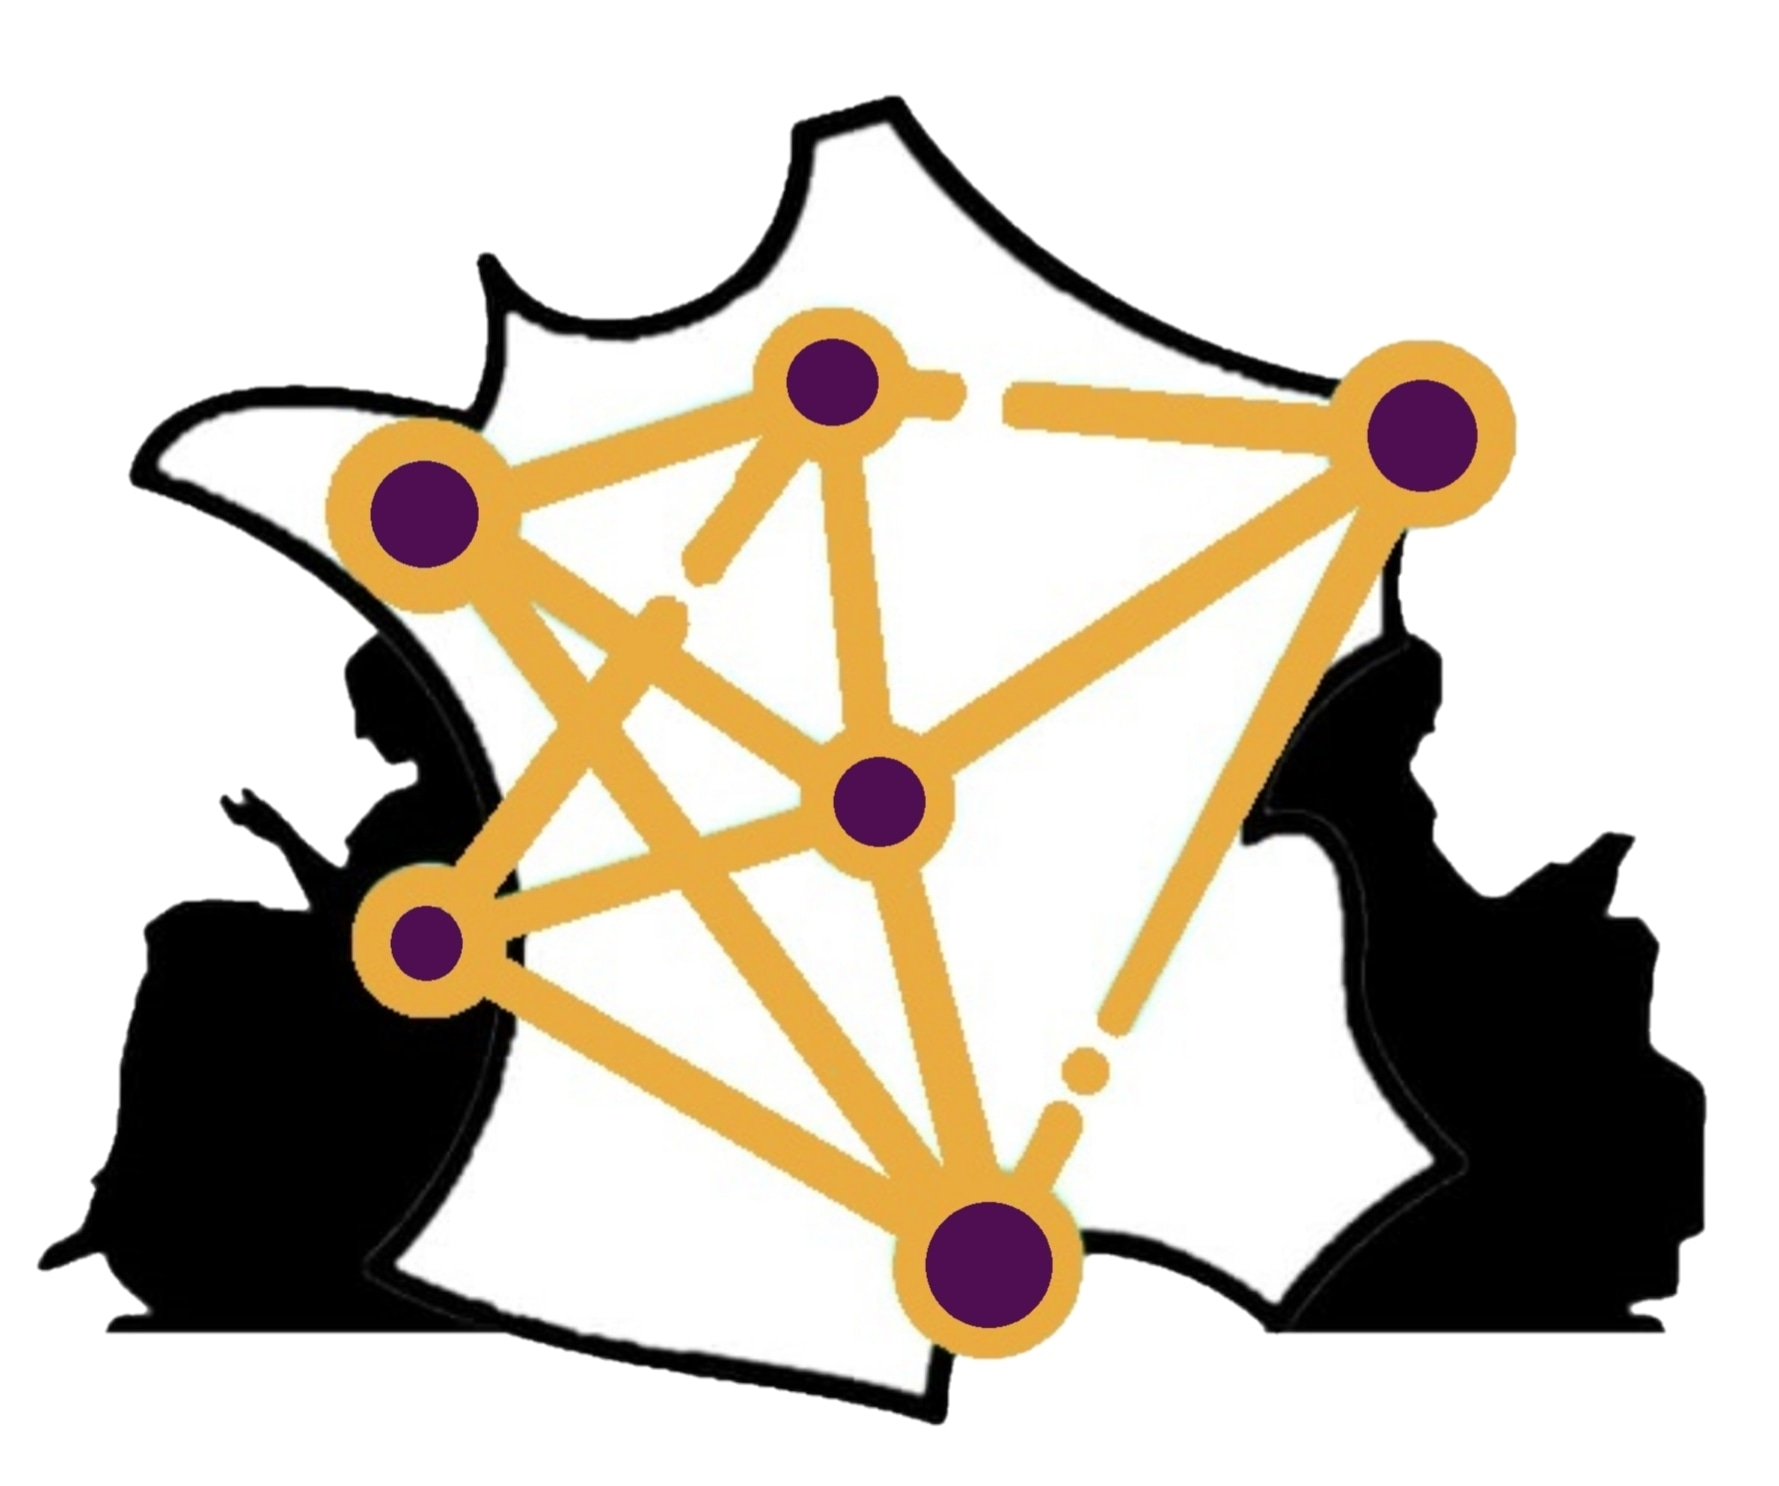
\includegraphics[height=0.8cm]{logo.jpg}} % 
}

\begin{document}
	\begin{frame}
		\titlepage
	\end{frame}
	\section{Généralités sur le séminaire}
	
	\begin{frame}
		\frametitle{Informations sur le cours}
		\textbf{Modalités :}
		\begin{itemize}
			\item 12 séances de 2 heures le mardi de 18h30 à 20h30. Le plus souvent plusieurs intervenants et intervenantes par séance (présentation sur le compte Instagram et le repo Github).
			\item \textbf{Validation} :
			\begin{enumerate}
				\item Assiduité (3 absences injustifiées maximum).
				\item Un exposé de 5 à 7 minutes sur 'l'actualité de la recherche en groupe.
				\item Un mini mémoire de 5 à 10 pages sur l'une des questions posées lors du cours.
			\end{enumerate}
		\end{itemize}
	\end{frame}
	
	\begin{frame}
		\frametitle{Déroulé du cours}
		\centering
		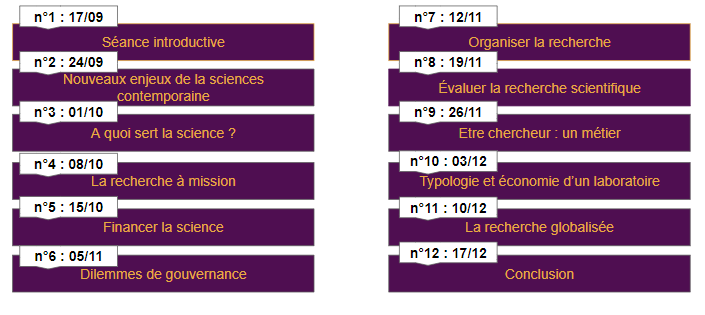
\includegraphics[scale=1]{Séances.PNG}
	\end{frame}
	
	\begin{frame}
		\frametitle{Exemple de présentation de l'actualité}
		\textbf{Bilan des investissements dans la recherche pour le sport\\de haut niveau\\}
		\textbf{\\Sources :}
		\begin{itemize}
			\item \href{https://www.aefinfo.fr/depeche/717186-jop-l-investissement-en-recherche-sur-la-performance-sportive-n-etait-pas-une-evidence-sylvie-retailleau}{"JOP : "L'investissement en recherche sur la performance sportive n'était pas une évidence" (Sylvie Retailleau)", AEF info, dépêche N°717186, Michèle Bargiel, 05/09/2024.}
			\item \href{https://www.enseignementsup-recherche.gouv.fr/fr/programme-prioritaire-de-recherche-ppr-sport-de-tres-haute-performance-92142}{"Programme Prioritaire de Recherche (PPR) Sport de très haute performance", MESR, 25/08/2023}
		\end{itemize}
	\end{frame}
	
	
	\begin{frame}
		\frametitle{Exemple de présentation de l'actualité}
		\textbf{Le PPR "Sport de très haute performance :}
		\begin{itemize}
			\item 20 M€ investis dans le cadre de France 2030 et gérés par l'ANR.
			\item 9 défis thématiques :
			\begin{multicols}{2}
				\begin{enumerate}
					\tiny
					\item l'équilibre de vie et l'environnement de l'athlète
					\item la prévention et le traitement des facteurs de risque
					\item cognition et préparation mentale
					\item les interactions homme-matériel et l'optimisation du matériel
					\item apprentissage et optimisation du geste sportif
					\item la quantification des charges d'entrainement
					\item les big data et l'intelligence artificielle au service de la performance
					\item la performance dans son environnement
					\item spécificités du domaine paralympique.
				\end{enumerate}
				\normalsize
			\end{multicols}
		\end{itemize}
	\end{frame}
	
	\begin{frame}
		\frametitle{Exemple de présentation de l'actualité}
		\textbf{Le PPR "Sport de très haute performance :}
		\begin{itemize}
			\item 12 projets soutenus via l'AAP de l'ANR :
			\begin{multicols}{2}
				\begin{enumerate}
					\tiny
					\item Neptune (natation et paranatation)
					\item Fulgure (sports de vitesse)
					\item D-Day (fatigue des nageurs)
					\item Team-Sports (management des sports collectifs)
					\item Paraperf (optimiser les équipements paralympiques)
					\item Du carbone à l'or olympique (carbone dans les sports de voile)
					\item HypoxPerf2024 (optimisation des entraînement en hypoxie)
					\item PerfAnalystics (approche scientifique de l'analyse vidéo)
					\item Revea (réalité virtuelle)
					\item TrainYourBrain (préparation mentale des escrimeurs)
					\item THPCA2024 (optimisation cyclisme et aviron)
					\item Best-Tennis (optimisation du service et du retour de service)
				\end{enumerate}
			\end{multicols}
		\end{itemize}
	\end{frame}
	\begin{frame}
		\frametitle{Exemple de présentation de l'actualité}
		\textbf{Sylvie Retailleau} : "Le bénéfice est des deux côtés : il s’agit d’un\\travail d’échange, de communication, de réseaux. Il va falloir continuer dans cette voie".
		\begin{center}
			\begin{tabularx}{0.8\textwidth} { 
					| >{\centering\arraybackslash}X 
					| >{\centering\arraybackslash}X
					| >{\centering\arraybackslash}X
					| >{\centering\arraybackslash}X | }
				\hline
				Sport & Projet & Médailles Tokyo 2020 & Médailles Paris 2024 \\
				\hline
				Natation & D-Day et Neptune  & 1 & 7 \\
				\hline
				Sports de voile & Du carbone à l'or olympique & 3 & 2  \\
				\hline
				Escrime & Train Your Brain & 5 & 7  \\
				\hline
				Cyclisme & THPCA2024 & 2 & 3 \\
				\hline
			\end{tabularx}
		\end{center}
	\end{frame}
	\begin{frame}
		\frametitle{Une perte d'avance}
		\centering
		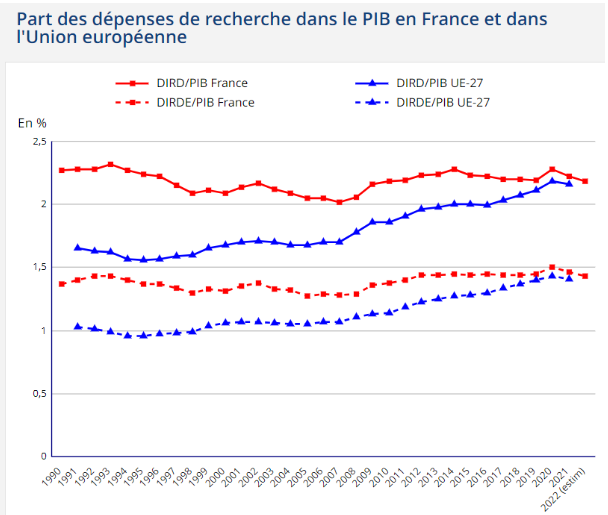
\includegraphics[scale=0.8]{DIRDA.PNG}
	\end{frame}
	\begin{frame}
		\frametitle{Une DIRDA qui stagne}
		\centering
		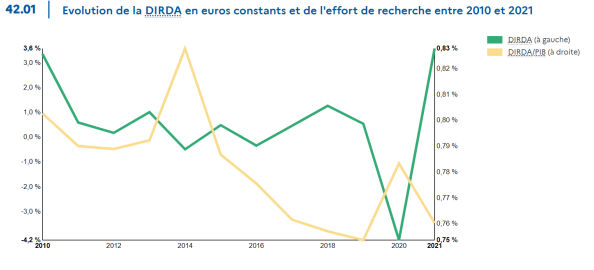
\includegraphics[scale=1.1]{DIRDA euro.PNG}
	\end{frame}
	\begin{frame}
		\frametitle{Une DIRDA qui stagne}
		\centering
		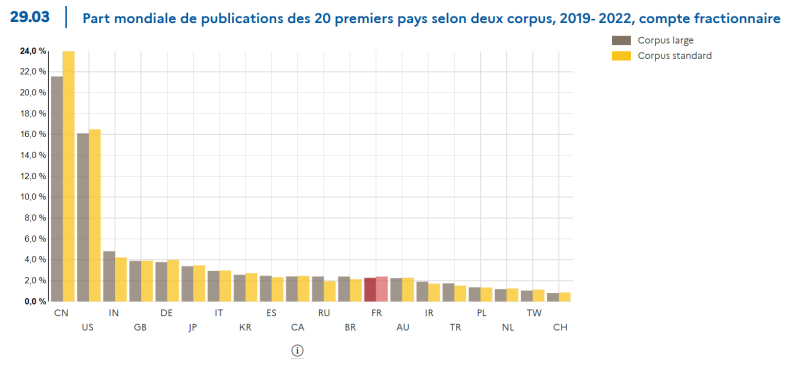
\includegraphics[scale=0.8]{Publications.PNG}
	\end{frame}
	
	\section{Science et la recherche ?}
	\begin{frame}
		\frametitle{Définitions : recherche}
		Il n'y a pas de définition légale et formelle de la recherche. Mais il y a une doctrine administrative depuis l'inscription des principes du \textbf{Manuel de Frascati} au BOFiP 2021.
		\begin{itemize}
			\item 3 niveaux de R\&D
			\item 5 critères systématiques
			\item Mais critiquables car (trop ?) limités.
		\end{itemize}
	\end{frame}
	\begin{frame}
		\frametitle{Définitions : recherche}
		\textbf{Les 3 niveaux de R\&D du Manuel de Frascati :}
		\begin{itemize}
			\item \textbf{Recherche fondamentale} : acquisition de connaissances sur les phénomènes sans envisager d'application.
			\item \textbf{Recherche appliquée} : acquisition de connaissances dirigée vers un but pratique déterminé.
			\item \textbf{Développement expérimental} : fondé sur les fruits de la recherche amont visant à l'acquisition de connaissances techniques et à déboucher sur de nouveaux produits ou procédés.
		\end{itemize}
	\end{frame}
	\begin{frame}
		\frametitle{Technology Readiness Level}
		\centering
		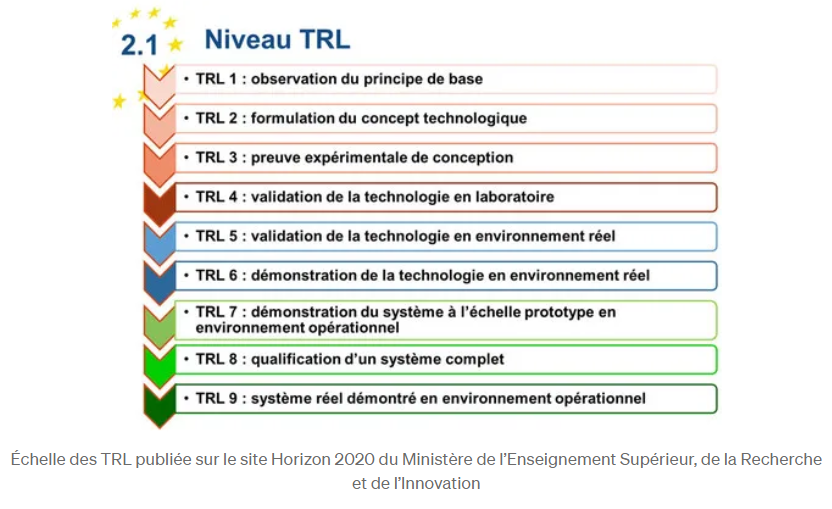
\includegraphics[scale=0.8]{TRL.PNG}
	\end{frame}
	\begin{frame}
		\frametitle{Définitions : recherche}
		\textbf{Les 5 critères du Manuel de Frascati :}
		\begin{itemize}
			\item \textbf{Nouveauté} : obtenir des résultats nouveaux.
			\item \textbf{Créativité} : reposer sur des notions et hypothèses originales.
			\item \textbf{Incertitude} : caractère incertain quant au résultat.
			\item \textbf{Systématicité} : planification et budgétisation.
			\item \textbf{Reproductibilité} : résultats que d'autres équipes doivent pouvoir reproduire.
		\end{itemize}
	\end{frame}
	\begin{frame}
		\frametitle{Définitions : science}
		\textbf{Michel Blay}, \textit{Dictionnaire des concepts philosophiques}, 2005 :
		\begin{multicols}{2}
			\begin{itemize}
				\small
				\item Clarté de la connaissance
				\item Démonstrations
				\item Raisonnements expérimentaux
				\item Analyse des sociétés et des faits humains
			\end{itemize}
			\normalsize
		\end{multicols}
		Critères de \textbf{scienticité} :
		\begin{multicols}{2}
			\small
			\begin{itemize}
				\item Déduction
				\item Reproductibilité
				\item Réfutabilité (Karl Popper)
				\item Cohérence (Willard Van Orman Quine)
				\item Simplicité (Guillaume d'Ockham)
				\item Responsabilité (Pierre Bourdieu)
			\end{itemize}
		\end{multicols}
		\normalsize
		\begin{center}
			Pourquoi faire une \textbf{science de la recherche} ?
		\end{center}
	\end{frame}
	\begin{frame}
		\frametitle{Déclinaisons des sciences}
		Sciences exactes, expérimentales, et sociales, ou classification\\d'Auguste Comte, etc. \textbf{Historiquement situé, méthodologiquement divers}.
		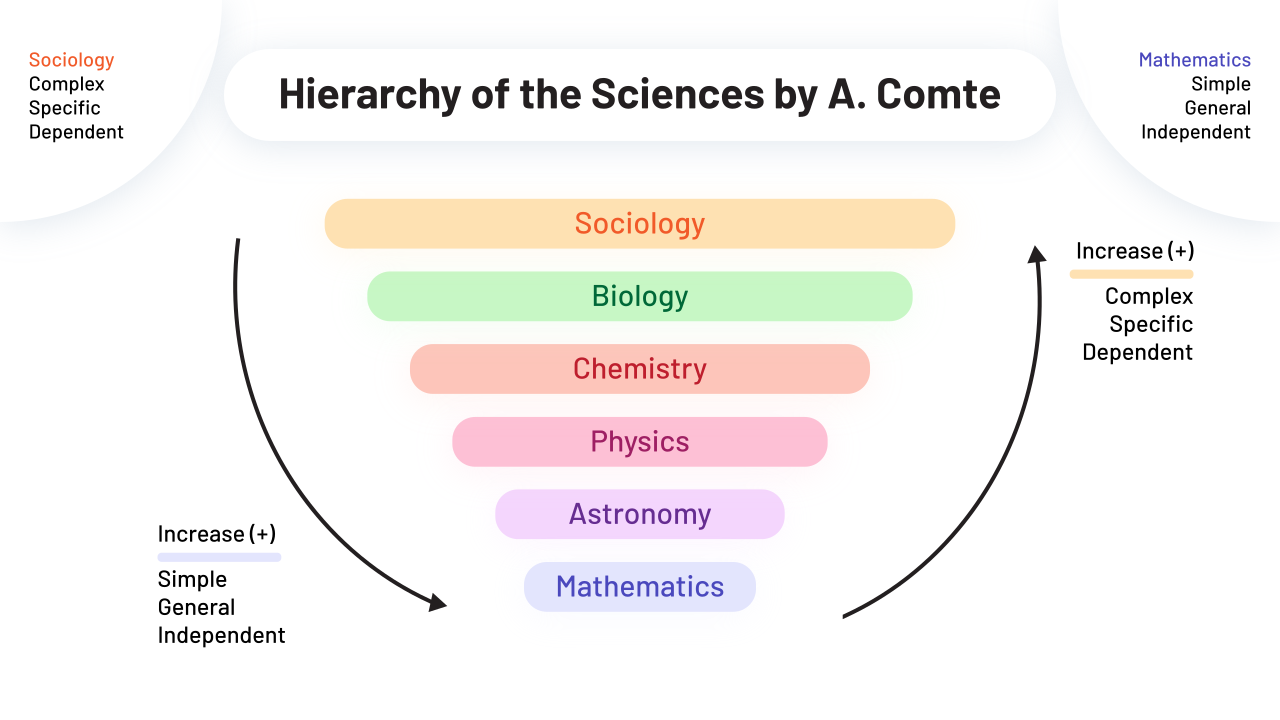
\includegraphics[scale=0.25]{Sciences.PNG}
	\end{frame}
	
	\section{Structure de l'ESR}
	\begin{frame}
		\frametitle{Objectifs de l'ESR}
		D'après la \textbf{loi de programmation de la recherche 2021-2030} :
		\begin{itemize}
			\item DIRD (DIRAD+DIRDE) doit être équivalente à 3\% du PIB.
			\item DIRDA doit être équivalente à 1\% du PIB.
			\item "[...] l'objectif d'accroître le rayonnement et de renforcer l'engagement de la France dans l'Europe de la recherche" (Article 1).
		\end{itemize}
		Objectifs supplementaires : recherche fondamentale, aides à la R\&D, innovation, valorisation.
	\end{frame}
	\begin{frame}{Institutions}
		Les institutions de la recherche :
		\begin{itemize}
			\item \textbf{Décisions et orientations} : MESR, Conseil stratégique de la recherche, Parlement, lieux de rencontres.
			\item \textbf{Programmation} : ANR, Bpifrance, Ademe, etc.
			\item \textbf{La recherche} : laboratoires publics, privés, communs, les grandes écoles et les universités.
			\item \textbf{L'évaluation} : le Haut conseil de l'évaluation de la recherche et de l'enseignement supérieur, IGF, SGPI, MESR.
		\end{itemize}
	\end{frame}
	\begin{frame}
		\frametitle{Les métiers de la recherche}
		\small
		\begin{multicols}{2}
			\begin{itemize}
				\item \textbf{Chargé de recherche} : missions de recherche et de formation.
				\item \textbf{Directeur de recherche} : conçoit, anime et coordonne les activités de recherche.
				\item \textbf{Ingénieur de recherche} : activités de R\&D appliquée, de formation, et d'encadrement de personnels techniques.
				\item \textbf{Ingénieur d'études} : rôle de chef de projet dans l'élaboration de nouvelles méthodes de productions, services, biens. Intervient à tous les stades des projets.
				\item \textbf{Assistants inégnieurs} : veillent à la préparation et au contrôle de l'exécution d'opérations techniques.
				\item \textbf{Techniciens de recherche} : mettent en oeuvre les méthodes et exécutent les opérations.
				\item \textbf{Beaucoup d'autres métiers} : institutions nationales et internationales, administration publique et privée de la recherche.
			\end{itemize}
			\normalsize
		\end{multicols}
	\end{frame}
	\section{La diversité des systèmes de recherche}
	\begin{frame}
		\frametitle{Exemples d'autres SR dans le monde}
		\textbf{L'Allemagne}
		\begin{itemize}
			\item \textbf{Acteurs extra-universitaires} : sociétés de recherche pluridiciplinaires avec un niveau de TRL (Max Planck pour la fondamentale, Fraunhofer pour l'appliquée et la valorisation), etc.
			\item \textbf{Acteurs universitaires} : au coeur du système de recherche. Ils reçoivent les fonds de l'Agence allemande de moyens pour la recherche. Ils collaborent entre eux, avec les sociétés de recherche, et le privé.
			\item \textbf{Caractéristiques} : plus indépendant que le système français, plus intégré, plus transparent au niveau des aides.
		\end{itemize}
	\end{frame}
	\begin{frame}
		\frametitle{Exemples d'autres SR dans le monde}
		\textbf{La Chine}
		\begin{itemize}
			\item \textbf{Acteurs privés} : peu développés, tournés vers la production, dépendants de l'étranger.
			\item \textbf{Acteurs publics} : 20 grands laboratoires pour les projets stratégiques, 533 laboratoires de recherche appliquée, 191 centres d'ingéniérie de recherche (valorisation).
			\item \textbf{Caractéristiques} : très centralisé, en phase de transformation vers le fondamental et l'énergie verte.
		\end{itemize}
	\end{frame}
	\begin{frame}
		\frametitle{Exemples d'autres SR dans le monde}
		\textbf{Les Etats-Unis}
		\begin{itemize}
			\item \textbf{Acteurs privés} : 2/3 des dépenses de R\&D (surtout industriels), contrats et plans avec les Departments, pôles d'excellence.
			\item \textbf{Acteurs publics} : financements fédéraux stables pour la recherche fondamentale,laboratoires et universités d'exception.
			\item \textbf{Caractéristiques} : hybride, liberté du fondamental, recherche à projets pour le reste, forte attractivité mais domination fragile.
		\end{itemize}
	\end{frame}
	\begin{frame}
		\frametitle{Espace européen de la recherche}
		\begin{itemize}
			\item Création dans les années 1980 pour coordonner les agences (CERN, ESO, ASE, etc.) via des \textbf{programmes cadre}. Travaille à \textbf{l'indépendance technologique} de l'Europe.
			\item Commission européenne, 2021, \textbf{Pacte pour la recherche et l'innovation en Europe} : valeurs, politiques, investissements.
			\item \textbf{Horizon Europe} : 95,5 Mds€ pour la période 2021-2027 afin de financer des projets communs et de venir en aide aux SR plus faibles.
			\item \textbf{Conseil européen de la recherche} : détermine les grandes orientations des programmes cadre, et assure la coordination des efforts des Etats.
		\end{itemize}
	\end{frame}
	\begin{frame}
		\frametitle{Interactions de ces SR avec la France}
		\textbf{La France dans Horizon Europe}
		\begin{itemize}
			\item 10,6\% des subventions obtenues en 2023
			\item 30\% des projets impliquant des français ont été financés
			\item la France participe à hauteur de 9,1\% du total
			\item le CNRS est l'organisme le plus financé
		\end{itemize}
	\end{frame}
	\section{Et la suite ?}
	\begin{frame}
		\frametitle{Les questions auxquelles on va répondre}
		\begin{itemize}
			\item Pourquoi faire de la recherche ?
			\item Que signifie s'investir dans la recherche, et devenir chercheuse ou chercheur ?
			\item Quels sont les modes d'organisation et de gouvernance de la recherche ?
			\item Que sait-on des réseaux de recherche ? Qu'aimerions-nous savoir ?
		\end{itemize}
	\end{frame}
	\begin{frame}{Liens}
		\begin{figure}
			\centering
			\begin{minipage}{.5\textwidth}
				\centering
				
\includegraphics[width=1\linewidth]{Insta.png}
			\end{minipage}%
			\begin{minipage}{.5\textwidth}
				\centering
				
\includegraphics[width=1\linewidth]{Github.jpg}
			\end{minipage}
		\end{figure}
	\end{frame}
\end{document}